%%%%%%%%%%%%%%%%%%%% author.tex %%%%%%%%%%%%%%%%%%%%%%%%%%%%%%%%%%%
%
% sample root file for your "contribution" to a proceedings volume
%
% Use this file as a template for your own input.
%
%%%%%%%%%%%%%%%% Springer %%%%%%%%%%%%%%%%%%%%%%%%%%%%%%%%%%


\documentclass{svproc}
%
% RECOMMENDED %%%%%%%%%%%%%%%%%%%%%%%%%%%%%%%%%%%%%%%%%%%%%%%%%%%
%

% to typeset URLs, URIs, and DOIs
\usepackage{url}
\usepackage[utf8]{inputenc}
\usepackage[brazil]{babel}
\usepackage{graphicx}
\def\UrlFont{\rmfamily}

\begin{document}
\mainmatter              % start of a contribution
%
\title{Sistema de Recomendação Baseado em Conteúdo Textual em Páginas Web}
%
\titlerunning{Hamiltonian Mechanics}  % abbreviated title (for running head)
%                                     also used for the TOC unless
%                                     \toctitle is used
%
\author{OMMITED}
%
\authorrunning{OMMITED} % abbreviated author list (for running head)
%
%%%% list of authors for the TOC (use if author list has to be modified)
\tocauthor{Ivar Ekeland, Roger Temam, Jeffrey Dean, David Grove,
Craig Chambers, Kim B. Bruce, and Elisa Bertino}
%
\institute{OMMITED\\
\email{OMMITED}
}

\maketitle              % typeset the title of the contribution

\begin{abstract}
Recommendation Systems has emerged to assist users against information overload in a environment where not all information is relevant or of interest to the user. Recommendation Systems came with the proposal of being an independent area in Computer Science, rather than filtering information, the focus is to recommend information based on preferences, tastes and interests surprising with new information and helping in the pursuit of the real need.
In this paper we present a recommendation system, that is compose by an middleware and a framework, for web environment based on textual content and the sequence of processes to arrive at a recommendation for the user, from the construction of profile (user interest) to the recommendation. This article also presents the strategies, technologies and areas related to Computer Science at each stage of the recommendation process.
% We would like to encourage you to list your keywords within
% the abstract section using the \keywords{...} command.
\keywords{recommendation system, tag cloud, profile user}
\end{abstract}
%
\section{Introduction}



\section{Sistemas de Recomendação}
Os sistemas de recomendação atuam em diferentes áreas, desde de Ciências Cognitivas, Teoria da Aproximação até Recuperação da Informação, com o intuito de prover indicação de conteúdo não classificado, somente com base em preferências do usuário~\cite{resnick1997recommender}.

Inicialmente, os sistemas de recomendação eram caracterizados como sistemas de filtragem colaborativa, em decorrência do primeiro sistema lançado, o~\emph{Tapestry}~\cite{goldberg1992using,resnick1994grouplens,medeiros2013estudo}. 
No entanto, foi pelo trabalho de Resnick e Varian~\cite{resnick1997recommender} que foi proposto o termo mais genérico ``Sistema de Recomendação'', sendo adotado por
não consistir em um produto de colaboração entre usuários, mas sim como foco na recomendação de informações~\cite{adomavicius2005toward,medeiros2013estudo}.

Segundo Gediminas e Alexander~\cite{adomavicius2005toward}, o problema de recomendação pode ser simplificado ao
problema da estimativa de classificação para as informações que ainda não foram
visualizados pelo usuário.

Desse modo, novamente, Gediminas e Alexander~\cite{adomavicius2005toward} definem um sistema de recomendação pela combinação dos conjuntos de todos os usuários~\emph{U}e de itens a serem recomendados~\emph{I}, mediados pela função~\emph{ü}, que mede quanto um item é relevante, cujo resultado da combinação~\emph{U x I} é ordenado em um conjunto~\emph{A}.
Resumidamente: 
$$u \in U, i'u = argmaxs \in Iu(\ddot u, i)$$

Em geral, na maioria dos casos o conjunto de itens analisados é muito inferior ao total. 
De modo análogo, a mesma relação pode ser mapeada como uma matriz esparsa, conforme apresentado na Figura~\ref{figure:esparsa}:

\begin{figure}[!ht]
\centering
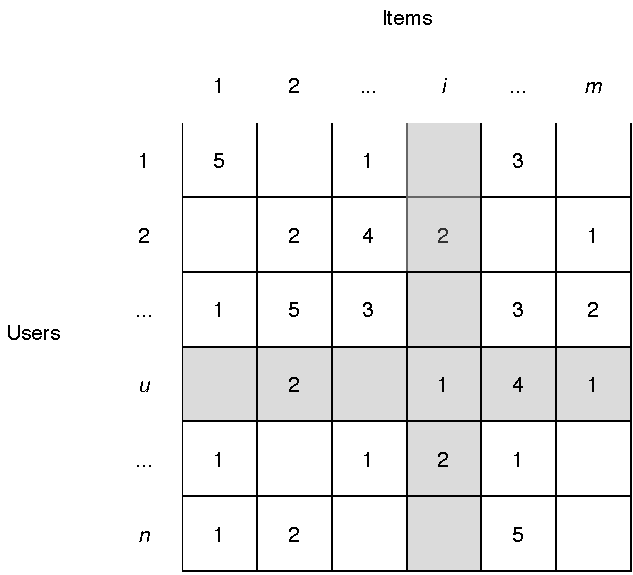
\includegraphics[width=.6\textwidth]{images/esparsa.pdf}
\caption{Conjunto esparso de recomendações.}
\label{figure:esparsa}
\end{figure}

A Figura~\ref{figure:esparsa} representa uma matriz de n usuários e m itens e cada célula $A(u,i)$ corresponde à uma avaliação do usuário u ao item i. 
O desafio é sempre superar a função~\emph{ü} para todo o conjunto~\emph{U x I} para que o usuário u tenha novas experiências e conhecimento de todo o conteúdo em que ele está inserido~\cite{adomavicius2005toward}.

De modo geral, os sistemas de recomendação atuam com base em um conjunto de atividades que iniciam na coleta de dados até a recomendação de itens, em que cada etapa é descrita brevemente nas Seções~\ref{section:coleta} a~\ref{section:tarefa}.

\subsection{Coleta de Dados}
\label{section:coleta}
A etapa inicial consiste na obtenção dos dados brutos, os quais atuam como base no processo de recomendação.
Essa atividade pode impactar diretamente no restante do processo, pois quanto específico ou gerais esses forem, consequentemente os resultados atuam de modo semelhante, os quais podem ocorrer em imprecisões ou erros de classificação.

A atividade pode ser executada de modos distintos, seja explícita ou implícita ao usuário, dentre as possíveis estratégias tem-se o monitoramento de atividades, solicitação de cadastros, navegação em páginas com~\emph{cookies} e a exibição de exemplos~\cite{cazella2010ciencia,reategui2006personalizaccao}.
A partir disso, a cada usuário é definido um perfil com base nas interações conduzidas.

%\subsection{Abordagem de Recomendação}
%\label{section:abordagem}

\subsection{Obtenção de Informação}
\label{section:obtencao}
Como segunda etapa, a partir dos dados brutos é necessário conduzir duas principais análises, sob perspectivos gerais e específicas de seu conteúdo.

Em uma análise geral, o processo de identificação de que tipo de informação e contexto que os dados são oriundos. 
Uma abordagem comum é a aplicação de técnicas de visualização de informação, como exemplo, a utilização de~\emph{Tag Clouds}, a qual permite a identificação dos principais conceitos relacionados ao conteúdo analisado com base na frequência dos termos~\cite{luis2017analise}.

Posteriormente, uma análise mais específica deve ser conduzia, de modo a identificar a relevância do elemento analisado, para isso são utilizados modelos baseados em Recuperação de Informação, permitindo a inter-conexão entre o provedor de informação e o consumidor~\cite{souza2006sistemas}.

Diferentes estratégias possuem base em Inteligência Artificial, as quais utilizam análise dos dados (utilização de palavras-chave indexadas), modelos lógicos (aplicação de regras booleanas ou lógica~\textit{fuzzy}), vetorais (frequência da ocorrência de elementos ou aplicação de redes neurais)~\cite{souza2006sistemas} ou probabilísticos (métodos de inferência ou predição)~\cite{khan2010review,silva2016}.
Esses modelos possuem em comum a utilização do perfil do usuário como base na realização da consulta~\cite{baeza1999modern,souza2006sistemas}.


\subsection{Tarefa de Recomendação}
\label{section:tarefa}
Por fim, cabe-se ao sistema de recomendação a condução na tomada de decisão pelo usuário. Nesse contexto, Silva~\cite{silva2016} aponta alguns objetivos e tarefas que devem ser cumpridos:
\begin{itemize}
    \item Anotações de Contexto: sugestão de opções que deveriam ser selecionadas.
    \item Seleção de Melhores Elementos: capacidade de identificar um conjunto limitado de potenciais elementos.
    \item Todos Elementos: recuperação de todos os elementos relacionados.
    \item Recomendação Sequencial: prover adequação nas sugestões com base nos passo a passo conduzido.
    \item Recomendação Quantitativa: fornecer recomendação para uma análise exploratória.
    \item Recomendação Confiável: estabelecer graus de confiança com base na qualidade das recomendações.
\end{itemize}
% ---- Bibliography ----
%
\bibliographystyle{splncs_srt}
\bibliography{references}
%
\end{document}
